\documentclass[a4paper]{article}
\usepackage{xgreek}
\usepackage{xunicode}
\usepackage{xltxtra}
\usepackage{setspace}
\usepackage{listings}
\usepackage{pdfpages}
\setlength{\parskip}{1ex}
\setlength{\topmargin}{0in}
\setlength{\oddsidemargin}{0in}
\setlength{\evensidemargin}{0in}
\setlength{\textheight}{9in}
\setlength{\textwidth}{6.25in}
\setmainfont[Mapping=tex-text]{GFS Didot}
\begin{document}
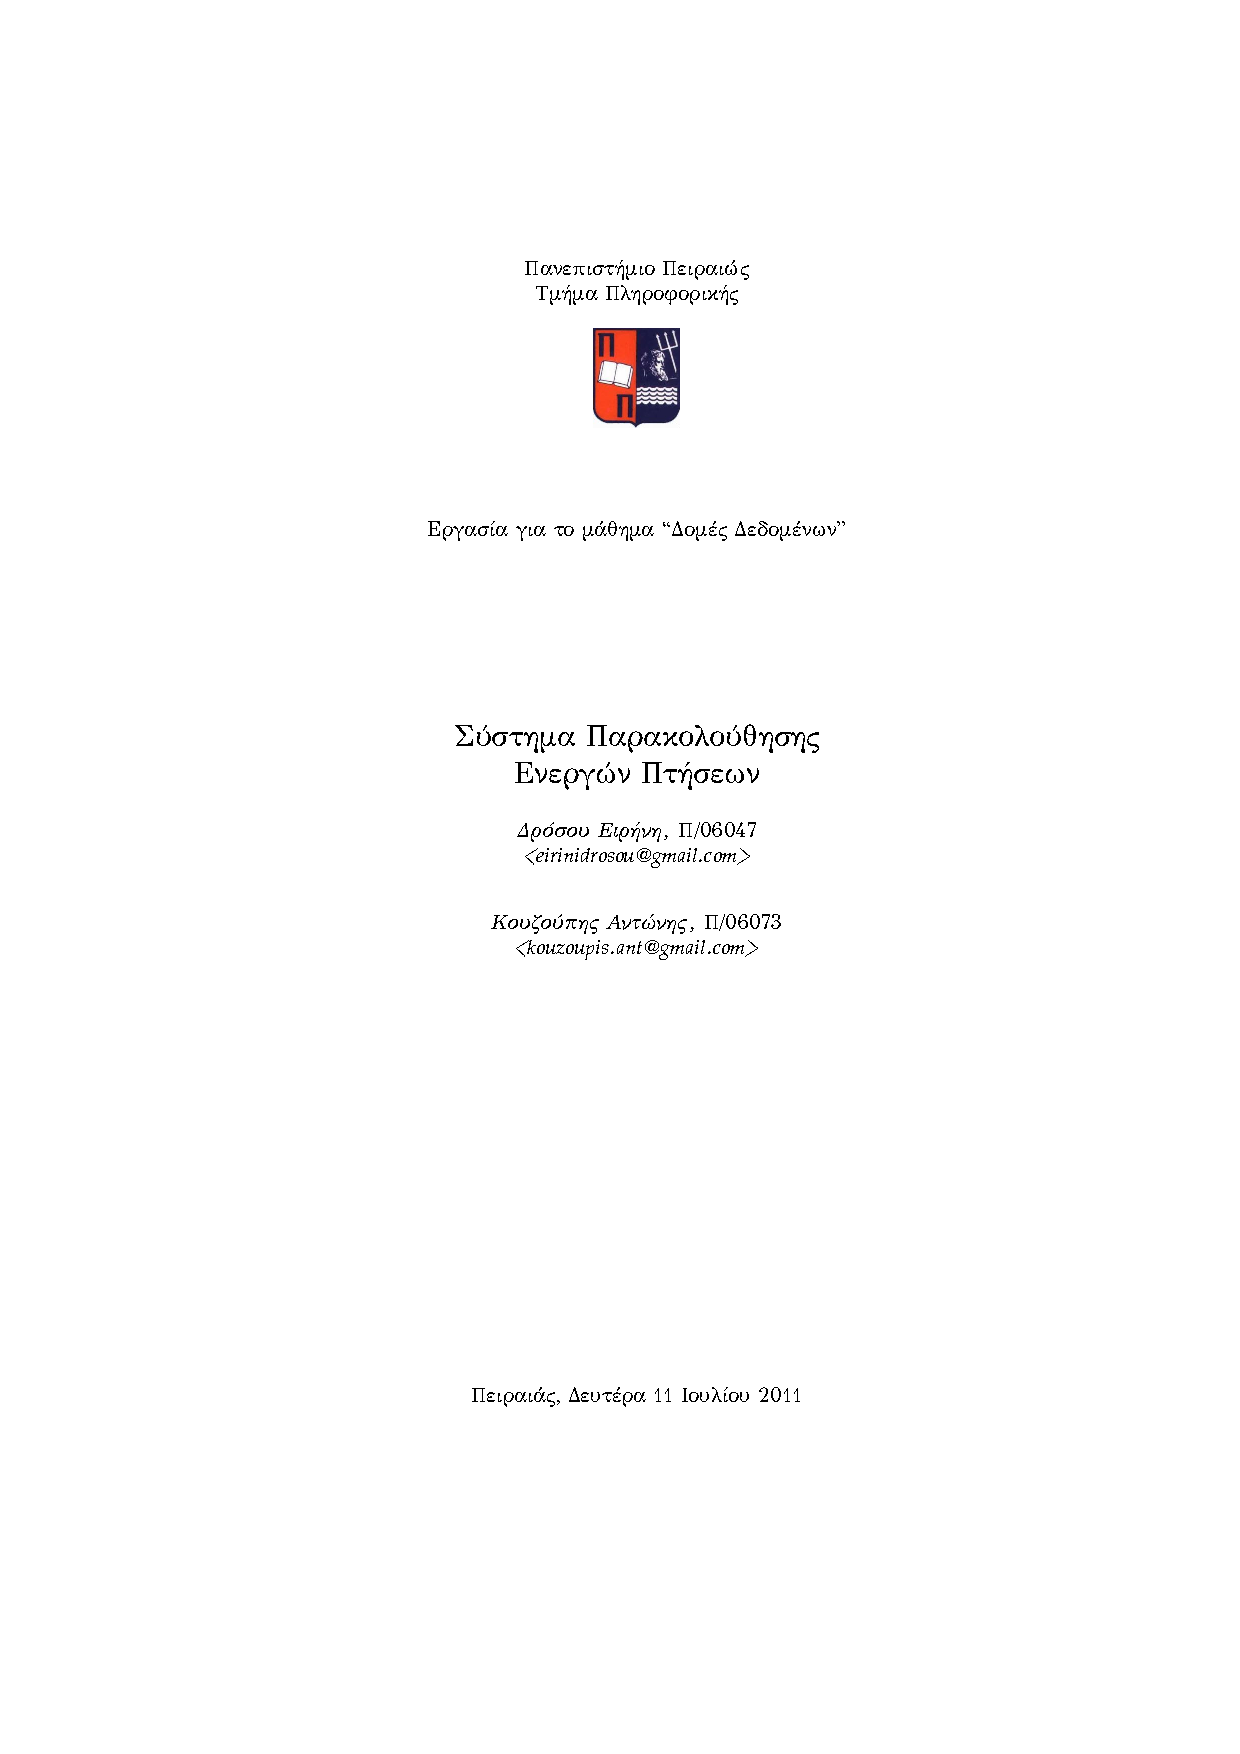
\includepdf[pages=-]{titlepage.pdf}
\tableofcontents
\newpage
\section{Εισαγωγή}
Η εφαρμογή υλοποιεί ένα απλοποιημένο σύστημα προβολής και διαχείρισης των
ενεργών πτήσεων. Υλοποιήθηκε στα πλαίσια της δεύτερης εργασίας του μαθήματος
\emph{Δομές Δεδομένων}. Υλοποιεί κάποιες λειτουργίες πάνω σε δυαδικό δένδρο
αναζήτησης. Η εφαρμογή είναι γραμμένη στη γλώσσα προγραμματισμού Java και οι 
δομές που χρησιμοποιήθηκαν δεν είναι οι built-in κλάσεις της γλώσσας αλλά
υλοποιημένες από εμάς. Δυστυχώς λόγω ακαδημαϊκών υποχρεώσεων δεν προλάβαμε να
υλοποιήσουμε το τέταρτο μέρος της εργασίας. Η εφαρμογή δεν χρησιμοποιεί κάποιο
είδος persistance καθώς δεν χρειαζόταν από την εργασία.
\section{Σχεδίαση}
Η εφαρμογή είναι χωρισμένη σε τρία βασικά λειτουργικά κομμάτια. Τα τρία
directories--packages της εφαρμογής είναι το business, το entities και το
structure. Κάθε ένα package περιέχει κώδικα ``ανεξάρτητο'' από τα άλλα packages.
Παρόλα αυτά χρειάζονται και τα τρία για να λειτουργήσει η εφαρμογή. Το πρώτο
πακέτο, το business, περιέχει τον πηγαίο κώδικα για το business logic. Τυπώνει
το μενού, συλλέγει τις πληροφορίες από το χρήστης, μετατρέπει τις raw
πληροφορίες σε μορφή χρήσιμη και καλεί τις κατάλληλες μεθόδους για λειτουργίες
πάνω στο δυαδικό δένδρο αναζήτησης. Στο δεύτερο πακέτο, το entities, υπάρχει ο
κώδικας για την υλοποίηση των οντοτήτων του συστήματος. Στη συγκεκριμένη
περίπτωση είναι οι πτήσεις. Τέλος στο πακέτο structures υπάρχουν οι κλάσεις των
δομών δεδομένων που χρησιμοποιήσαμε οι οποίες προφανώς υλοποιούν τις δομές αλλά
και κάποιες λειτουργίες πάνω σε αυτές.

Αναλυτικές πληροφορίες υπάρχουν και στο \emph{JavaDoc} που συνοδεύει την εργασία
αλλά και στον πηγαίο κώδικα.

\subsection{business package}
Το συγκεκριμένο πακέτο περιέχει τις κλάσεις \emph{Business}, \emph{Main} και
\emph{Printer}.

Η κλάση \emph{Business} περιέχει τρεις βασικές μεθόδους. Η μία είναι για να
φορτώνει κάποιες demo πτήσεις στο σύστημα, η δεύτερη προετοιμάζει τα raw
δεδομένα που εισάγει ο χρήστης και καλεί τις κατάλληλες μεθόδους για την
προσθήκη μιας νέας πτήσης και τέλος η τρίτη μέθοδος χρησιμοποιείται για την
αναζήτηση των ενεργών πτήσεων σε ένα συγκεκριμένο χρονικό διάστημα.

Η κλάση \emph{Main} είναι το entry point της εφαρμογής. Μέσω μεθόδων της κλάσης
\emph{Printer} τυπώνει το κεντρικό μενού, τα υπο--μενού και συλλέγει τις
πληροφορίες από τον χρήστη.

Τελευταία είναι η κλάση \emph{Printer} που αποτελείται από μεθόδους που
προορίζονται αποκλειστικά στην εκτύπωση των διάφορων μενού και ``ερωτήσεων''
προς το χρήστη.

\subsection{entities package}
Το πακέτο \emph{entities} περιέχει την κλάση \emph{Flights}.

Η κλάση \emph{Flights} κρατάει όλες τις λεπτομέρειες για μία πτήση. Ο
πληροφορίες που κρατάει είναι ο κωδικός πτήσης, η ώρα αναχώρησης και η ώρα
άφιξης. Ουσιαστικά ένα instance της κλάσης αυτής αντιπροσωπεύει μία πτήση.
Επίσης έχει διάφορες άλλες μεθόδους για να θέτουμε και να διαβάζουμε τις τιμές
των παραπάνω μεταβλητών (getters \& setters). Τέλος υπάρχει μία μέθοδος για την
εκτύπωση των λεπτομερειών μιας πτήσης.

\subsection{structure package}
Το πακέτο αυτό περιέχει τις κλάσεις \emph{BinarySearchTree} και
\emph{SimplyLinkedList}.

Η κλάση \emph{BinarySearchTree} υλοποιεί αρχικά ένα Δυαδικό Δένδρο Αναζήτησης
καθώς και κάποιες επιπλέον λειτουργίες. Κάθε κόμβος του δένδρου αποθηκεύει
instances της κλάσης \emph{Flights}, δηλαδή αποθηκεύει πτήσεις. Κάθε κόμβος
επίσης έχει ένα πεδίο \textbf{MaxArr} το οποίο κρατάει τη μέγιστη ώρα άφιξης του
υποδένδρου του. Στην κλάση αυτή υπάρχει και η κλάση \emph{Node} που
αντιπροσωπεύει τους κόμβους του δένδρου. Κρατάει πληροφορίες για τον αριστερό
κόμβο--παιδί, τον δεξιό κόμβο--παιδί, το πεδίο \textbf{MaxArr} και φυσικά τα
δεδομένα. Έχει μεθόδους για την εισαγωγή, διαγραφή, αναζήτηση ενός κόμβου και
εκτύπωση σε ενδοδιάταξη του δένδρου.

H κλάση \emph{SimplyLinkedList} υλοποιεί μία μονά συνδεδεμένη λίστα που
επίσης χρησιμοποιεί Generics. Αποτελείται και αυτή από δύο κλάσεις, η μία είναι η
\emph{SNode} που κρατάει διάφορες πληροφορίες για ένα κόμβο όπως τη τιμή του
κόμβου και τον επόμενο κόμβο. Έχει επίσης κάποιες μεθόδους για την προσπέλαση
των στοιχείων αυτών. Η κλάση \emph{SimplyLinkedList} υλοποιεί κάποιες
λειτουργίες της μονά συνδεδεμένης λίστας όπως την προσθήκη ενός κόμβου είτε στην
αρχή, είτε στο τέλος είτε κάπου ενδιάμεσα, τη διαγραφή ενός κόμβου, μέθοδο για
την παίρνουμε το μέγεθος της λίστας, μέθοδο για να βλέπουμε αν η λίστα είναι
άδεια και μία μέθοδο που τυπώνει τις τιμές όλων των κόμβων της λίστας. Η λίστα
χρησιμοποιείται ως στοίβα (stack) για τις λειτουργίες της εισαγωγής και
διαγραφής.

\subsection{Δομή Εφαρμογής}
Όπως αναφέραμε η εφαρμογή κρατάει κάποιες πτήσεις σε μία δομή δυαδικού δένδρου
αναζήτησης και εκτελούμε κάποιες λειτουργίες σε αυτές. Μία πτήση χαρακτηρίζεται
από τον κωδικό πτήσης, την ημερομηνία αναχώρησης και την ημερομηνία άφιξης. Στο
δένδρο η ταξινόμηση γίνεται με βάση την ημερομηνία αναχώρησης. Επίσης κάθε
κόμβος στο δένδρο έχει ένα ειδικό field με όνομα \textbf{MaxArr}. Αυτό το πεδίο
κρατάει την μέγιστη ημερομηνία άφιξης του δένδρου κάτω από αυτό, δηλαδή του
υποδένδρου του. Αυτό το πεδίο βοηθάει για διάφορες αναζητήσεις ώστε να μπορούμε
να αποφασίζουμε να μην επισκεπτόμαστε κάποια υποδένδρα. Με αυτό τον τρόπο
γλιτώνουμε συγκρίσεις. Προφανώς όταν γίνεται κάποια εισαγωγή ή διαγραφή, οι
κόμβοι του δένδρου θα πρέπει να επανατοποθετηθούν στη σωστή θέση και να
υπολογιστεί ξανά το πεδίο \textbf{MaxArr}.

\section{Επεξήγηση Λειτουργίας}
Η εφαρμογή είναι γραμμένη σε Java οπότε για να τρέξει ή να γίνει compile
χρειαζόμαστε το Java Runtime Enviroment. Τα εκτελέσιμα είναι αρχειοθετημένα σε
ένα archive τύπου jar για ποιο εύκολη εκτέλεση. Για να ξεκινήσουμε την εφαρμογή
αρκεί να πάμε στον κατάλογο που είναι το αρχείο \emph{DataStruct2.jar} και να
εκτελέσουμε \emph{java -jar DataStruct2.jar}. Αυτό θα μας εμφανίσει το κεντρικό
μενού της εφαρμογής απ' όπου μπορούμε να κάνουμε τις επιλογές μας. Το κεντρικό
μενού θα εμφανίζεται μετά από κάθε λειτουργία εκτός αν επιλέγουμε την Έξοδο από
την εφαρμογή. Το entry point του συστήματος είναι η κλάση Main που φορτώνει
κάποιες demo πτήσεις.

\subsection{Add Flight}
Η πρώτη επιλογή είναι για τη προσθήκη μιας πτήσης στην εφαρμογή. Επιλέγοντας
λοιπόν την πρώτη επιλογή, μας εμφανίζεται ένα prompt για να εισάγουμε τα
χαρακτηριστικά της πτήσης. Αφού τα εισάγουμε, η ημερομηνία αναχώρησης και
ημερομηνία άφιξης μετατρέπονται σε χρόνο EPOCH. Έπειτα δημιουργείται ένα νέο
instance της κλάσης \emph{Flights} και καλείται η μέθοδος \emph{add} της κλάσης
\emph{BinarySearchTree}. Αυτή η μέθοδος αποφασίζει ποιο είναι το σωστό σημείο
στο δένδρο για να μπει και ρυθμίζει κατάλληλα τους δείκτες προς το αριστερό και
δεξιό παιδί. Σε ένα stack κρατάει τους κόμβους που έκανε traverse μέχρι να βρει
τη σωστή θέση ώστε μετά να ελέγξει αν χρειάζεται επανυπολογισμός του πεδίου
\textbf{MaxArr} σε κάθε ένα κόμβο από το stack.

\subsection{List Flights}
Δεύτερη επιλογή είναι για την προβολή όλων των πτήσεων. Η επιλογή αυτή καλεί τη
μέθοδο \emph{toString} της κλάσης \emph{BinarySearchTree} και αφού μετατρέψει το
δένδρο σε μία λίστα με ενδοδιάταξη, τυπώνει όλα τα περιεχόμενα.

\subsection{Delete Flight}
Με την επιλογή \emph{Delete Flight} μπορεί ο χρήστης να διαγράψει μία πτήση από
το σύστημα. Προφανώς αφού διαγραφεί ένας κόμβος, το δυαδικό δένδρο αναζήτησης θα
πρέπει να έχει τη σωστή δομή και το πεδίο \textbf{MaxArr} να έχει τη σωστή τιμή
σε όλους τους κόμβους. Αρχικά ο χρήστης δίνει ένα κωδικό πτήσης, καλείται η
μέθοδος \emph{delFlight} της κλάσης \emph{BinarySearchTree} όπου βρίσκει σε ποιο
κόμβο αντιστοιχεί ο συγκεκριμένος κωδικός πτήσης. Έπειτα καλείται η μέθοδος
\emph{remove} της ίδιας κλάσης όπου διαγράφει τον κόμβο και αποφασίζει ποιος
κόμβος θα πάρει τη θέση του στο δένδρο. Επίσης κρατάει σε μία λίστα όλους τους
κόμβους που έχουν γίνει traversed μέχρι τον κόμβο προς διαγραφεί έτσι ώστε μετά
να ελέγξει αν χρειάζεται αλλαγή το πεδίο \textbf{MaxArr}.

\subsection{Search within a period}
Επόμενη επιλογή είναι η αναζήτηση πτήσεων σε εξέλιξη σε ένα συγκεκριμένο χρονικό
διάστημα. Ο χρήστης δίνει την αρχή και το τέλος του χρονικού διαστήματος και
επιστρέφονται οι πτήσεις που άρχισαν στο διάστημα αυτό ή ολοκληρώθηκαν στο
διάστημα αυτό. Αφού ο χρήστης δώσει την αρχή και το τέλος καλείται η μέθοδος
\emph{searchFlight} της κλάσης \emph{Business}, μετατρέπει τις ημερομηνίες σε
χρόνους EPOCH και καλεί τη μέθοδο \emph{searchPeriod} της κλάσης
\emph{BinarySearchTree}. Η μέθοδος αυτή επιστρέφει μία λίστα με όλες τις πτήσεις
που είναι σε εξέλιξη στη συγκεκριμένη χρονική περίοδο και τελικά τις τυπώνει.

\subsection{Exit}
Τελευταία επιλογή είναι η \emph{Exit} με την οποία μπορούμε να τερματίσουμε και
να βγούμε από την εφαρμογή.

\section{Περιεχόμενα CD}
Στο CD που συνοδεύει το παρόν εγχειρίδιο υπάρχουν τα παρακάτω:
\begin{description}
\item[src] Ο πηγαίος κώδικας της εφαρμογής. Περιέχει τρεις καταλόγους που
αντιστοιχούν στα τρία πακέτα. Το κάθε πακέτο έχει τον κώδικα από τις κλάσεις
του.
\item[doc] Το Javadoc της εφαρμογής. Περιγραφή της λειτουργίας κάθε μεθόδου της
εφαρμογής. Μέσα στον κατάλογο αυτό υπάρχει το αρχείο \emph{index.html} το οποίο
το ανοίγετε με ένα browser. (Σε ορισμένους browsers ίσως χρειαστεί να θέσετε με
το χέρι την κωδικοποίηση σε UTF-8)
\item[Documentation.pdf] Το παρόν εγχειρίδιο.
\item[DataStruct2.jar] jar archive το οποίο περιέχει τον εκτελέσιμο κώδικα.
\item[README] Αρχείο με πληροφορίες για την εκτέλεση της εφαρμογής.
\end{description}
\end{document}
